\subsection*{Solution to Spring 2012, \#1}\label{s121}
\subsubsection*{Solution to $1a$}
We have
\begin{align*}
\dot{H}(x, y) &= (-\sin x  \cos y)\dot{x} + \cos x(-\sin y) \dot{y}\\
&= (-\sin x\cos y)(\sin y\cos x) + (-\cos x\sin y)(-\cos y\sin x) = 0.
\end{align*}
Therefore $H(x, y)$ is conserved.
\hfill\qed

\subsubsection*{Solution to $1b$}
As $\frac{\pr }{\pr x}(\sin y\cos x) + \frac{\pr}{\pr y}(-\cos y\sin x) = 0$, the system is Hamiltonian.
Therefore all fixed points are either centers (elliptic fixed points) or saddles (hyperbolic fixed points).
The fixed points are when $\sin y\cos x = 0$ and $\cos y \sin x = 0$. Thus the fixed points are of type:
\begin{enumerate}
\item[$(1)$] $\{(n\pi, m\pi): n, m \in \Z\}$
\item[$(2)$] $\{((n + \frac{1}{2})\pi, (m + \frac{1}{2})\pi): n, m \in \Z\}$.
\end{enumerate}
The Jacobian is
$$J(x, y) = \pmat{-\sin x\sin y}{\cos x\cos y}{-\cos x\cos y}{\sin x\sin y}.$$
Therefore the Jacobian for the fixed points of Type $(1)$ is $\smat{0}{(-1)^{n+ m}}{(-1)^{n + m + 1}}{0}$.
This matrix has eigenvalues $\pm i$. Since the system is Hamiltonian, all fixed points
of Type $(1)$ are elliptic.

The Jacobian for the fixed points of Type $(2)$ is $\smat{(-1)^{n + m + 1}}{0}{0}{(-1)^{n + m}}$. This matrix
has eigenvalues $\pm 1$ and hence as the system is Hamiltonian, the fixed points of Type $(2)$ are hyperbolic.
The phase portrait is as follows:

\begin{center}
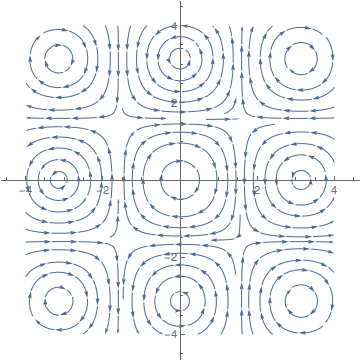
\includegraphics[scale=0.60]{./_Figures/S121.png}
\end{center}
\hfill\qed

\subsubsection*{Solution to $1c$}
When close to the elliptic fixed points, the ODE system behaves like the system
$$\vct{x}{y}' = \pmat{0}{(-1)^{n + m}}{(-1)^{n + m  + 1}}{0}\vct{x}{y}.$$
Therefore
$$\frac{dy}{dx} = \frac{y'}{x'} = \frac{(-1)^{n + m + 1}x}{(-1)^{n + m}y} = -\frac{x}{y}.$$
Solving this gives $x^{2} + y^{2} = C$ for some constant $C$. Therefore the trajectories
near elliptic fixed points are circles and so have period $2\pi$.

On the other hand, when close to hyperbolic fixed points, the ODE system behaves like the system
$$\vct{x}{y}' = \pmat{(-1)^{n + m + 1}}{0}{0}{(-1)^{n + m}}\vct{x}{y}.$$
Therefore
$$\frac{dy}{dx} = \frac{y'}{x'} = \frac{(-1)^{n + m}y}{(-1)^{n + m + 1}x} = -\frac{y}{x}.$$
Solving this gives $xy = C$ for some constant $C$. Therefore as we get arbitrarily close to
a hyperbolic fixed point, we never return and so the period is infinite (we get sent
to another hyperbolic fixed point).
\hfill\qed

\subsection*{Solution to Spring 2012, \#2}\label{s122}

\subsubsection*{Solution to $2a$}
There's probably a typo in the initial conditions. It should probably read
$$ u(x,0) = \frac{\d u}{\d t} (x,0) = 0 $$
as opposed to a partial derivative with respect to $x$.

With this in mind, the solution to the inhomogeneous wave equation comes directly from applying Duhamel's principle, which yields
$$ u(x,t) = \frac{1}{2} \int_0^t \int_{x-(t-s)}^{x+(t-s)} f(y,s) \, dy ds $$ \hfill\qed

\subsubsection*{Solution to $2b$}
\begin{rem}
This problem is a bit confusing since $\Delta$ is a triangle which looks like it depends on inputs $x, t$.
To make our analysis clear, we will assume for the rest of this problem $\Delta$ is a given fixed triangle with vertices that
will not depend on the inputs of any functions that appear in the problem
(for concreteness, we can take $\Delta$ to be, for example, the triangle with vertices $(1, 1), (0, 0)$, and $(2, 0)$). \hfill\qed
\end{rem}

With the above remark in mind, we now solve the problem. Using Duhamel's principle, we can write the solution to the PDE in implicit form:
$$u(x,t) =  \frac{1}{2} \int_0^t \int_{x-(t-s)}^{x+(t-s)} f(y,s) - a(y,s) u_s(y,s) - b(y,s) u_y (y,s) - c(y,s) u(y,s) \, dy ds $$
Hence, a solution to the PDE is a fixed point of the operator
$$ F(\varphi)(x,t) := \frac{1}{2}  \int_0^t \int_{x-(t-s)}^{x+(t-s)} f(y,s) - a(y,s) \varphi_s(y,s) - b(y,s) \varphi_y (y,s) - c(y,s) \varphi (y,s) \, dy ds $$
where $\varphi \in \text{BC}^{1,1} (\R \times (0,\infty) \to \R)$, the set of bounded continuous functions with bounded continuous first derivatives in both variables from $\R \times (0,\infty) \to \R$, which is a complete metric space under the norm defined by
$$ \|u\| :=  \|u(x,t)\|_{\infty} + \left| \left| \frac{\d u}{\d x} (x,t) \right| \right|_{\infty} + \left| \left| \frac{\d u}{\d t} (x,t) \right| \right|_{\infty} $$
where $\| \cdot \|_{\infty}$ is the sup norm. Now, define $h_{\varphi}(y,s) := f(y,s) - a(y,s) u_s(y,s) - b(y,s) u_y (y,s) - c(y,s) u(y,s)$, which is the integrand of the functional defined above. Before we prove that $F$ is a contraction mapping, observe, by the fundamental theorem of calculus,
$$ \frac{\d F}{\d x}(\varphi)(x,t) = \frac{1}{2} \int_0^t h_{\varphi}(x+(t-s),s) - h_{\varphi}(x-(t-s),s) \, ds $$
$$ \frac{\d F}{\d t}(\varphi)(x,t) = \frac{1}{2} \int_0^t h_{\varphi} (x+(t-s),s) + h_{\varphi}(x-(t-s),s) \, ds $$
Define  $C := \max \{ \|a(x,t)\|_{0,\Delta}, \|b(x,t)\|_{0,\Delta}, \|c(x,t)\|_{0,\Delta}\}$. Let $0 < t < T$, where we choose $T < \min \left\{ 2, \frac{1}{6(1+C)} \right\}$. We compute
\begin{align}
\nonumber \|F(\varphi)\| &\leq \frac{1}{2}t^2(  \|f\|_{0,\Delta} + C \|\varphi\|) + 2t( \|f\|_{0,\Delta} + C \|\varphi\|)   \\
\nonumber &< \frac{1}{2}T^2 + 2T(\|f\|_{0,\Delta} + C \|\varphi\|) \\
\label{s12bound} &< \frac{1}{2(1+C)} (\|f\|_{0,\Delta} + C \|\varphi\|)
\end{align}
Define $V := \{ \varphi \in \text{BC}^{1,1} (\R \times (0,\infty) \to \R) \, : \, \|\varphi\| \leq \|f\|_{0,\Delta} \}$. Since $V$ is a closed subset of $\text{BC}^{1,1} (\R \times (0,\infty) \to \R)$, $V$ is complete. We will now show that $F : V \to V$ and that $F$ is a contraction on $V$. In other words, we will show $F(\varphi) \in V$ for all $\varphi \in V$, and for any $\varphi, \phi \in V$, $\|F(\varphi) - F(\phi)\|_{\infty} \leq \alpha \|\varphi-\phi\|_{\infty}$ for some $\alpha \in [0,1)$.

\vspace{0.2cm}

First, we show that $F(\varphi) \in V$ for all $\varphi \in V$. By \eqref{s12bound},
$$\|F(\varphi)\| < \frac{1}{2(1+C)} (\|f\|_{0,\Delta} + C \|f\|_{0,\Delta}) = \frac{1}{2} \|f\|_{0,\Delta} \leq \|f\|_{0,\Delta} $$
Thus, $F(\varphi) \in V$ for all $\varphi \in V$. Next, let $\varphi, \phi \in V$. Then,
\begin{align*}
	\|F(\varphi) - F(\phi)\| &= \frac{1}{2} \left| \left| \int_0^t \int_{x-(t-s)}^{x+(t-s)} h_{\varphi}(y,s) - h_{\phi}(y,s) \, dy ds \right| \right|  \\
	&\leq \frac{1}{2} t^2 C \| \varphi - \phi\| \\
	&< \frac{1}{6} \|\varphi-\phi\|
\end{align*}
Thus, $F$ is a contraction on $V$. Therefore, there exists a unique fixed point in $V$. Since fixed points of $F$ are solutions to the PDE, there exists a unique solution to the PDE if $T$ is chosen sufficiently small. Also, since $f, a, b$, and $c$ are all smooth functions, the solution will be as well.

\vspace{0.4cm}

To show the estimate, we notice
\begin{align*}
	\|u\|_{1,\Delta} &= \|F(u)\|_{1,\Delta} \\
	&= \max_{(y,\tau) \in \Delta} \left( |F(u)| + \left| \frac{\d F}{\d x}(u) \right| + \left| \frac{\d F}{\d t}(u) \right| \right) \\
	&\leq \|F(u)\|_{\infty} + \left| \left| \frac{\d F}{\d x}(u) \right| \right|_{\infty} + \left| \left| \frac{\d F}{\d t}(u) \right| \right|_{\infty} \\
	&\leq \frac{1}{2} t^2 (\|f\|_{0,\Delta} + C \|u\| ) + 2t (\|f\|_{0,\Delta} + C \|u\|) \\
	&= \left( \frac{1}{2} t^2 + 2t \right) (\|f\|_{0,\Delta} + C\|u\|)
\end{align*}
Since $u \in V$, we have
$$ \|u\|_{1,\Delta} \leq \left( \frac{1}{2} t^2 + 2t \right) (\|f\|_{0,\Delta} + C\|f\|_{0,\Delta}) $$
Because we chose $t$ such that $t \leq \min \left\{ 2, \frac{1}{6(1+C)} \right\}$, we have
\begin{align*}
\|u\|_{1,\Delta} &\leq 3t (1+C)\|f\|_{0,\Delta}\\
&\leq \frac{1}{2} \|f\|_{0,\Delta}
\end{align*}
Therefore, the estimate holds.
\hfill\qed

\subsection*{Solution to Spring 2012, \#3}\label{s123}
\subsubsection*{Solution to $3a$}
We have $-sU' + U^{2}U' = \vep U''$ which can be written as $-sU' + (\frac{1}{3}U^{3})' = \vep U''.$
Integrating both sides gives
$$-sU + \frac{1}{3}U^{3} = \vep U' + C_{1}$$
for some constant $C_{1}$.
\hfill\qed

\subsubsection*{Solution to $3b$}
Since $u(+\infty) = U_{R}$ and $u(-\infty) = U_{L}$,
$$-sU_{R} + \frac{1}{3}U_{R}^{3} = C_{1}$$
and
$$-sU_{L} + \frac{1}{3}U_{L}^{3} = C_{1}.$$
Therefore
$$-sU_{R} + sU_{L} + \frac{1}{3}U_{R}^{3} - \frac{1}{3}U_{L}^{3} = 0.$$
Factoring out a $U_{R} - U_{L}$ (which is nonzero) shows that
$$s = \frac{1}{3}(U_{R}^{2} + U_{R}U_{L} + U_{L}^{2})$$ and hence
$$C_{1} = -sU_{R} + \frac{1}{3}U_{R}^{3} = -\frac{1}{3}U_{R}^{2}U_{L} - \frac{1}{3}U_{L}^{2}U_{R}.$$
Since $-sU + \frac{1}{3}U^{3} = \vep U' + C_{1}$,
$-3sU + U^{3} = 3\vep U' + 3C_{1}$ and hence
$$-(U_{R}^{2} + U_{R}U_{L} + U_{L}^{2})U + U^{3} = 3\vep U' - U_{R}^{2}U_{L} - U_{L}^{2}U_{R}.$$
Isolating the $3\vep U'$ terms yields that
$$3\vep U' = (U - U_{R})(U - U_{L})(U + U_{L} + U_{R}).$$
Thus $U$ can be solved for using partial fraction decomposition. Suppose we had $A, B, C$ such that
\begin{align}\label{s123beq1}
\frac{1}{(U - U_{R})(U - U_{L})(U + U_{L} + U_{R})} = \frac{A}{U - U_{R}} + \frac{B}{U - U_{R}} + \frac{C}{U + U_{L} + U_{R}}.
\end{align}
Then
$$A\log|U - U_{R}| + B\log|U - U_{L}| + C\log|U + U_{L} + U_{R}| = \frac{1}{3\vep}s + \wt{C}$$
for some constant $\wt{C}$ (here we have used $\log$ to denote natural log). Thus as long as we can find $A, B, C$ we have a
solution. We have
\begin{align*}
1 = A(U - U_{L})(U + U_{L} + U_{R}) + B(U - U_{R})(U + U_{L} + U_{R}) + C(U - U_{L})(U - U_{R}
\end{align*}
for all $U$. Therefore
\begin{align*}
B(U_{L} - U_{R})(2U_{L} + U_{R}) &= 1\\
A(U_{R} - U_{L})(2U_{R} + U_{L}) & = 1\\
C(-2U_{L} - U_{R})(-2U_{R} - U_{L}) &= 1.
\end{align*}
Thus $A, B, C$ exist if $U_{L} - U_{R} \neq 0$, $2U_{L} + U_{R} \neq 0$, and $2U_{R} + U_{L} \neq 0$.
\hfill\qed

\subsection*{Solution to Spring 2012, \#4}\label{s124}
We will write $X \lsm Y$ if there exists
a positive constant $C$ such that $X \leq CY$. We will write $X \lsm_{f} Y$ if there exists a positive constant $C_{f}$ depending
only on $f$ such that $X \leq C_{f}Y$.
\subsubsection*{Solution to $4a$}
This is similar to the proof of the fundamental solution for the Laplacian. Let $L:= \Delta + k^{2}U$ and $u(x) = \int_{\R^{3}}E(y)f(x - y)\, dy$.
We want to show that $Lu(x) = -f(x)$. We have
\begin{align*}
Lu(x) = \int_{\R^{3}\bs B(0, \vep)}E(y)Lf(x - y)\, dy + \int_{B(0, \vep)}E(y)Lf(x - y)\, dy.
\end{align*}
Observe that
\begin{align*}
\abb{\int_{B(0, \vep)}\frac{e^{ik|y|}}{4\pi|y|}(\Delta_{x}f(x - y) + k^{2}f(x - y))\, dy} \lsm_{f}\int_{B(0, \vep)}\frac{1}{|y|}\, dy \lsm_{f}\int_{0}^{\vep}\frac{1}{r}r^{2}\, dr\lsm_{f} \vep^{2} \rightarrow 0
\end{align*}
as $\vep \rightarrow 0$. Furthermore,
\begin{align*}
\int_{\R^{3}\bs B(0, \vep)}E(y)Lf(x - y)\, dy = \int_{\R^{3}\bs B(0, \vep)}E(y)\Delta_{x}f(x - y)\, dy + \int_{\R^{3}\bs B(0, \vep)}E(y)k^{2}f(x - y)\, dy.
\end{align*}
We have
\begin{align*}
&\int_{\R^{3}\bs B(0, \vep)}E(y)\Delta_{x}f(x - y)\, dy= \int_{\R^{3}\bs B(0, \vep)}E(y)\Delta_{y}f(x - y)\, dy\\
&\quad= -\int_{\R^{3}\bs B(0, \vep)}\nabla E(y) \cdot \nabla_{y}f(x - y)\, dy + \int_{\pr B(0, \vep)}\frac{\pr f}{\pr\nu}(x - y)E(y)\, d\sigma_{y}\\
&\quad= \int_{\R^{3}\bs B(0, \vep)}\Delta E(y)f(x - y)\, dy - \int_{\pr B(0, \vep)}\frac{\pr E}{\pr \nu}(y)f(x - y)\, d\sigma_{y} + \int_{\pr B(0, \vep)}\frac{\pr f}{\pr\nu}(x - y)E(y)\, d\sigma_{y}
\end{align*}
where $\nu$ is the inner normal for $B(0, \vep)$ (which is the outer normal for $\R^{3}\bs B(0, \vep)$.
Since $\Delta E + k^{2}E = 0$ away from $0$,
\begin{align*}
\int_{\R^{3}\bs B(0, \vep)}E(y)Lf(x - y)\, dy = \int_{\pr B(0, \vep)}\frac{\pr f}{\pr \nu}(x - y)E(y) - \frac{\pr E}{\pr \nu}(y)f(x - y)\, d\sigma_{y}.
\end{align*}
Notice that
\begin{align*}
\abb{\int_{\pr B(0, \vep)}\frac{\pr f}{\pr \nu}(x - y)E(y)\, d\sigma_{y}} \lsm_{f} \int_{\pr B(0, \vep)}\frac{1}{\vep}\, d\sigma_{y} \lsm_{f} \vep \rightarrow 0
\end{align*}\
as $\vep \rightarrow 0$. Finally observe that as $\pr_{j}E = \frac{1}{4\pi}e^{ik|x|}(\frac{ikx_{j}}{|x|^{2}} - \frac{x_{j}}{|x|^{3}})$,
$$\nabla E(x) = \frac{e^{ik|x|}}{4\pi}\bigg(\frac{ikx}{|x|^{2}} - \frac{x}{|x|^{3}}\bigg).$$
Since $\nu$ is the inner normal for $B(0, \vep)$, $\nu = -x/|x|$ and hence
$$\frac{\pr E}{\pr \nu}(x) = \nu \cdot \nabla E = -\frac{e^{ik|x|}}{4\pi}\bigg(\frac{ik}{|x|} - \frac{1}{|x|^{2}}\bigg).$$
Thus
\begin{equation}
\begin{aligned}\label{s124eq1}
-\int_{\pr B(0, \vep)}\frac{\pr E}{\pr \nu}(y)f(x - y)\, d\sigma_{y}&= \int_{\pr B(0, \vep)}\frac{e^{ik\vep}}{4\pi}\bigg(\frac{ik}{\vep} - \frac{1}{\vep^{2}}\bigg)f(x -y)\, d\sigma_{y}\\&= \frac{ik\vep e^{ik\vep}}{4\pi \vep^{2}}\int_{\pr B(0, \vep)}f(x - y)\, d\sigma_{y} - \frac{e^{ik\vep}}{4\pi \vep^{2}}\int_{\pr B(0, \vep)}f(x - y)\, d\sigma_{y}.
\end{aligned}
\end{equation}
Since
$$\frac{1}{4\pi\vep^{2}}\int_{\pr B(0, \vep)}f(x - y)\, d\sigma_{y} \rightarrow f(x)$$
as $\vep \rightarrow 0$, it follows that the right hand side of \eqref{s124eq1} tends to $-f(x)$ as $\vep \rightarrow 0$. Therefore $Lu = -f$ as desired.
\hfill\qed

\subsubsection*{Solution to $4b$}
Integration by parts yields
\begin{align*}
\int_{\pr B(0, R)}\frac{\pr u}{\pr \nu}E(x_{0} - y) &- \frac{\pr E(x_{0} -y)}{\pr \nu}u\, d\sigma_{y}\\
&= \int_{B(0, R)}\Delta u E(x_{0} - y)\, dy - \int_{B(0, R)}u\Delta E(x_{0} - y)\, dy\\
&= \int_{B(0, R)}E(x_{0} - y)(\Delta u + k^{2}u) - u(\Delta E(x_{0} - y) + k^{2}E(x_{0} - y))\, dy\\
&= -\int_{B(0, R)}u(-\delta (x_{0} - y))\, dy = u(x_{0}).
\end{align*}
\hfill\qed

\subsubsection*{Solution to $4c$}
Fix arbitrary $x_{0}$ and let $R$ be such that $R > |x_{0}|$. Then
$$u(x_{0}) = \int_{\pr B(0, 2R)}\frac{\pr u}{\pr \nu}E(x_{0} - y) - u\frac{\pr E(x_{0} - y)}{\pr \nu}\, d\sigma_{y}.$$
Note that
\begin{align*}
\frac{\pr E(x_{0} - y)}{\pr \nu} = \nu \cdot \nabla(E(x_{0} - y)) = -\nu \cdot (\nabla E)(x_{0} - y) = \frac{e^{ik|x_{0} - y|}}{4\pi}\bigg(\frac{ik}{|x_{0} - y|} - \frac{1}{|x_{0} - y|^{2}}\bigg)
\end{align*}
and hence
\begin{align*}
u(x_{0}) &= \int_{\pr B(0, 2R)}(o(1/R) + iku)E(x_{0} - y) - u\frac{e^{ik|x_{0} - y|}}{4\pi}\bigg(\frac{ik}{|x_{0} - y|} - \frac{1}{|x_{0} - y|^{2}}\bigg)\, d\sigma_{y}\\
&=\int_{\pr B(0, 2R)}o(\frac{1}{R})E(x_{0} - y) + O(\frac{1}{R})\frac{e^{ik(x_{0} - y)}}{4\pi|x_{0} - y|^{2}}\, d\sigma_{y}.
\end{align*}
Thus
\begin{align*}
|u(x_{0})| &\lsm \int_{\pr B(0, 2R)}o(\frac{1}{R})\frac{1}{|x_{0} - y|} + O(\frac{1}{R})\frac{1}{|x_{0} - y|^{2}}\, d\sigma_{y}\\
&\lsm \int_{\pr B(0, 2R)}o(\frac{1}{R})\frac{1}{R} + O(\frac{1}{R})\frac{1}{R^{2}}\, d\sigma_{y} \lsm o(\frac{1}{R})R + O(\frac{1}{R}) \rightarrow 0
\end{align*}
as $R \rightarrow \infty$. Therefore since $x_{0}$ was arbitrary, $u \equiv 0$.
\hfill\qed

\subsection*{Solution to Spring 2012, \#5}\label{s125}
We will assume that $\beta$ does not vanish on $\pr\Om$ and $\pr\Om$ is sufficiently smooth.
\subsubsection*{Solution to $5a$}
Integration by parts yields that
\begin{align*}
\int_{\Om}v_{x_{k}}\beta(x)u_{x_{k}}\, dx = -\int_{\Om}v(\beta(x)u_{x_{k}})_{x_{k}}\, dx + \int_{\pr\Om}v\beta(x)u_{x_{k}}\nu^{k}\, d\sigma.
\end{align*}
Thus
\begin{align*}
\int_{\Om}\nabla v\cdot (\beta\nabla u)\, dx = -\int_{\Om}v\nabla \cdot (\beta\nabla u)\, dx + \int_{\pr\Om}v\beta\frac{\pr u}{\pr \nu}\, d\sigma.
\end{align*}
We have
\begin{equation}
\begin{aligned}\label{s125eq1}
-\int_{\Om}v\nabla \cdot (\beta \nabla u)\, dx &- \int_{\Om}vf \, dx+ \int_{\pr\Om}\ld v\, d\sigma\\
&+ \int_{\pr\Om}v\beta \frac{\pr u}{\pr \nu}\, d\sigma + \int_{\pr\Om}\mu u \, d\sigma- \int_{\pr \Om}\mu g\, d\sigma  = 0.
\end{aligned}
\end{equation}
Taking $\mu = 0$ and arbitrary $v \in H_{0}^{1}(\Om)$ in \eqref{s125eq1} yields that
$$-\nabla \cdot (\beta \nabla u) = f$$ in $\Om$. Then from \eqref{s125eq1} it follows that for all $v \in H^{1}(\Om)$,
\begin{align}\label{s125eq2}
\int_{\pr\Om}v(\ld + \beta \frac{\pr u}{\pr \nu})\, d\sigma + \int_{\pr\Om}\mu(u - g)\, d\sigma = 0.
\end{align}
Next take $\mu = 0$ in \eqref{s125eq2}. Since $v \in H^{1}(\Om)$ is arbitrary, we have
$$\beta \frac{\pr u}{\pr\nu} = -\ld$$ on $\pr\Om$. Finally, taking $v \in H_{0}^{1}(\Om)$ in \eqref{s125eq2} and using arbitrariness
of $\mu$ shows $u = g$ on $\pr\Om$. Therefore $u$ is the solution of the Dirichlet problem
\begin{align*}
\begin{cases}
-\nabla \cdot (\beta\nabla u) = f & \text{ in } \Om\\
u = g & \text{ on }\pr\Om\\
\beta\nabla u \cdot \nu =-\lambda & \text{ on } \pr\Om.
\end{cases}
\end{align*}
\hfill\qed

\subsubsection*{Solution to $5b$}
We have $\beta(\pr u/\pr\nu) = \beta(\pr w/\pr \nu)$ on $\pr\Om$. Therefore $\beta(\frac{\pr u}{\pr \nu} - \frac{\pr w}{\pr\nu}) = 0$
on $\pr\Om$. If we assume that $\beta$ does not vanish on $\pr\Om$, then $\nabla u \cdot \nu = \nabla w \cdot \nu$ on $\pr\Om$.
Therefore $\nabla u = \nabla w$ on $\pr\Om$ which implies that $w = g + c$ for some $c$ on $\pr\Om$.
\hfill\qed

\subsection*{Solution to Spring 2012, \#6}\label{s126}

\subsubsection*{Solution to $6a$}

Before starting, note that we are looking for the classical/strong solution to the PDE. This means shocks cannot occur, which is why the problem says that the solution can only be defined for some $x$ and $t$.

\vspace{0.4cm}

We use method of characteristics to obtain the following ODEs:
\begin{equation}
	\label{s126eq1} \dot{t}(s) = 1, \quad t(0) = 0
\end{equation}
\begin{equation}
	\label{s126eq2} \dot{x}(s) = z(s), \quad x(0) = x_0
\end{equation}
\begin{equation}
	\label{s126eq3} \dot{z}(s) = 0, \quad z(0) = x_0^2
\end{equation}
Solving \eqref{s126eq1} and \eqref{s126eq3} yields
$$ t(s) = s, \quad \text{and} \quad z(t) = x_0^2 $$
respectively. Then, solving \eqref{s126eq2} yields
\begin{equation}
	\label{s126eq4} x(t) = x_0^2 t + x_0
\end{equation}
Solving \eqref{s126eq4} for $x_0$ will gives
$$ x_0 = \frac{-1 \pm \sqrt{1+4xt}}{2t} $$
In order to determine which sign we pick to define $x_0$, we examine the limit as $t \to 0^+$ of $x_0$. Note that
$$ \lim_{t \to 0^+}  \frac{-1 + \sqrt{1+4xt}}{2t} = \lim_{t \to 0^+} \frac{x}{\sqrt{1+4xt}} = x \quad \text{and} \quad \lim_{t \to 0^+} \frac{-1 - \sqrt{1+4xt}}{2t} = -\infty $$
The first case is the one that we want, so we have
$$ x_0 = \frac{-1 + \sqrt{1+4xt}}{2t} $$
Now, we'll determine for what $x$ and $t$ will we have a strong solution. Consider two characteristics that start at $x=a \geq 0$ and $x=b \geq 0$, namely the characteristics $x = a^2 t + a$ and $ x = b^2 t + b$, respectively. These characteristics crash at $(x,t) = \left( \frac{ab}{a+b}, \frac{-1}{a+b} \right)$, which we can ignore because $t = -1/(a+b) < 0$. Thus, our solution will be defined on at least the set $\{(x,t) \, | \, x \geq 0, t > 0 \}$.

\vspace{0.4cm}

Now, consider the characteristic starting at $x=a < 0$, which will be $x = a^2 t + a$. Because of the slopes of the characteristics that start on the negative $x$-axis, the characteristic $x = a^2t + a$ will crash into another characteristics that starts immediately to the left or right of $a$. From our work above, we already know when and where characteristics crash, so with $a$ fixed, let's send $b$ to $a$ to see where and when the characteristics crash:
$$ x = \lim_{b \to a} \frac{ab}{a+b} = \frac{a}{2}, \quad \text{and} \quad t = \lim_{b \to a} \frac{-1}{a+b} = \frac{-1}{2a} $$
Putting these two expressions together yields
$$t = \frac{-1}{4x} $$
This implies that characteristics that start right next to each other on the negative $x$-axis will crash on the contour $4xt + 1 = 0$. Thus, we have for our strong solution
$$ u(x,t) = \frac{1 + 2xt - \sqrt{1+4xt}}{2t^2} $$
for $x  > -\frac{1}{4t}$ and $t > 0$. Note that $\lim_{t \to 0^+} u(x,t) = x^2$, so this choice of $u$ satisfies the initial condition. \qed


\subsubsection*{Solution to $6b$}
$$ u_x(x,t) = \frac{1}{t} \left( 1 - \frac{1}{\sqrt{1+4xt}} \right) $$
Hence, the magnitude of the derivative of the strong solution becomes infinite when $1+4xt = 0$. In other words, the magnitude of the derivative of our strong solution blows up as we approach the left-hand side boundary of the domain for which our strong solution is defined. This makes sense because that's where all of the characteristics crash. \qed



\subsubsection*{Solution to $6c$}

Recall that, from our work above, the following determines our solution:
$$ x(t) = u_0(x_0) t + x_0, \quad \text{and} \quad z(t) = u_0(x_0) $$
Hence, with our new initial condition, we know that
$$ u(x,t) = \frac{1}{4} \quad \text{when} \quad x - \frac{1}{4} t < -\frac{1}{2} \quad \Leftrightarrow \quad t > 4x+2$$
and
$$ u(x,t) = \frac{1}{4} \quad \text{when} \quad x - \frac{1}{4} t > \frac{1}{2} \quad \Leftrightarrow \quad t < 4x-2$$
This wasn't explicitly stated above, but we always have $t > 0$. Based on our work above, we also know that
$$ u(x,t) = \frac{1 + 2xt - \sqrt{1+4xt}}{2t^2} $$
for $x_0 \in [0,1/2)$, and no characteristics that start in the interval $[0,1/2)$ will crash with the characteristics that start in the interval $(1/2, \infty)$. Hence, everything boils down to what happens when characteristics start in the interval $(-1/2,0)$.

\vspace{0.4cm}

Earlier, we discovered that characteristics that start on the negative $x$-axis will crash along the contour $1+4xt=0$. Because $t=4x+2$ is a characteristic that starts at $x = -1/2$ for initial data $u_0(x) = x^2$, all we need to do is figure out when this line intersects the contour $1+4xt=0$. Some straightforward algebra yields the point $(x,t) = (-1/4, 1)$. Hence, the ODE that describes the trajectory of the shock is
$$ \frac{ \frac{1}{2} \left[ \left( \frac{1}{4} \right)^2 - \left( u_r \right)^2 \right]}{\frac{1}{4} - u_r} = \dot{x}(t), \quad x(1) = -\frac{1}{4}, \quad \text{where} \quad u_r = \frac{1 + 2xt - \sqrt{1+4xt}}{2t^2}. $$ \qed

\subsection*{Solution to Spring 2012, \#7}\label{s127}
Let
$$\phi(r) := \frac{1}{2\pi r}\int_{\pr B(x, r)}u(y)\, d\sigma_{y} = \frac{1}{2\pi}\int_{\pr B(0, 1)}u(x + ry)\, d\sigma_{y}.$$
We have
\begin{align*}
\phi'(r) = \frac{1}{2\pi}\int_{\pr B(0, 1)}\nabla u(x + ry)\cdot y\, d\sigma_{y} = \frac{1}{2\pi r}\int_{\pr B(x, r)}\nabla u(z) \cdot \frac{z - x}{r}\, d\sigma_{z}.
\end{align*}
Since the outer unit normal for $\pr B(x, r)$ is $(z - x)/r$, we have $\nabla u(z) \cdot (\frac{z - x}{r}) = \frac{\pr u}{\pr \nu}$.
Thus
$$\phi'(r) = \frac{1}{2\pi r}\int_{\pr B(x, r)}\frac{\pr u}{\pr \nu}\, d\sigma_{z} = \frac{1}{2\pi r}\int_{B(x, r)}\Delta u\, dz > 0.$$
Therefore $\phi$ is an increasing function of $r$. It follows that for any $\vep > 0$,
$$u(x) = \lim_{r\rightarrow 0}\frac{1}{2\pi r}\int_{\pr B(x, r)}u(y)\, d\sigma_{y} = \lim_{r \rightarrow 0}\phi(r) \leq \phi(\vep) = \frac{1}{2\pi \vep}\int_{\pr B(x, \vep)}u(y)\, d\sigma_{y}.$$
\hfill\qed

\subsection*{Solution to Spring 2012, \#8}\label{s128}
We use separation of variables to find all bounded solutions. Suppose $u(x,y) = X(x)Y(y)$. Plugging this into the PDE yields
\begin{align*}
	 X''(x)Y(y) + X(x)Y''(y) + k^2 X(x)Y(y) = 0 \quad &\implies \quad \frac{X''(x)}{X(x)} + \frac{Y''(y)}{Y(y)} + k^2 = 0 \\
	 &\implies \quad  \frac{X''(x)}{X(x)} + k^2 = -  \frac{Y''(y)}{Y(y)} = \lambda
\end{align*}
Hence, we must solve the following ODEs:
$$ X''(x) + (k^2 - \lambda) X(x) = 0, \quad \text{and} \quad Y''(y) + \lambda Y(y) = 0 $$
After examining the ODE for $x$, it becomes apparent that we require $|\lambda| < k^2$. If $|\lambda| \geq k^2$, then we only have the zero solution. Taking $|\lambda| < k^2$, we have
$$ X(x) = A \sin(\sqrt{k^2 - \lambda} x) + B \cos (\sqrt{k^2 - \lambda} x) $$
Applying the boundary conditions, we get $B = 0$ and
$$ \sqrt{k^2 - \lambda} = n \quad \implies \quad \lambda = k^2 - n^2 $$
for $|n| \leq  k$. Thus, for such $n$,
$$ X_n(x) = A_n \sin (nx) $$
It then follows that the ODE for $y$ is
$$ Y''(y) + (k^2 - n^2) Y(y) = 0 $$
Solving this yields
$$ Y_n(y) = C_n \sin (\sqrt{k^2 - n^2} y) + D_n \cos( \sqrt{k^2 - n^2} y) $$
for $|n| < k$ and
$$ Y_n(y) = D_n $$
for $|n| = k$. Therefore, we have
$$ u(x,y) = \sum_{|n| < k} \sin(nx) \left[ E_n \sin(\sqrt{k^2-n^2} y) + F_n \cos(\sqrt{k^2-n^2} y) \right] + \sum_{|n| = k} G_n \sin(nx) $$
where $E_n, F_n, G_n$ are finite sequences of constants. \qed
